\subsection{LEM - Lattice-Element-Method}
\Authors{Amir Shoarian Sattari (CAU)}
The application of the lattice element in modeling the fracture initiation and propagation in geomaterials has been well established \cite{Liuetal2007, Pradoetal2003, vanMieretal2002}. The main advantage of the LEM over other numerical methods is the ability to model the stress redistribution and concentration upon the fracking process. The application of the LEM is extended to model the heat transfer in cemented geomaterials \cite{Sattarietal2017} as well as non-cohesive granular particles \cite{Rizvietal2018b}. The thermo-mechanical lattice model based on the integration of the interface element is able to model the expansion and shrinkage processes during the heating and cooling cycles \cite{Sattarietal2019b}. The LEM is also implemented to model the foam concrete behavior under dynamic loading \cite{Rizvietal2018a}. In the past decade, using the dual lattice model to simulate the coupled hydro-mechanical loadings in geomaterials has developed \cite{Grassl2009}. In these models, the dual mesh grid for the fluid transport is generated. The short description of the implemented coupled thermo-hydro-mechanical lattice method is given below.

\subsubsection*{Discretization of the domain}
\label{Section:DiscretizationLattice}

The domain is discretized into a series of Voronoi cells to represent the individual particles or a continuum depending on the purpose of the investigation. With the application of the vectorized random lattice (VRL), the irregularity factor known as the randomness factor ($\alpha_{R}$), which varies between 0 and 1, is introduced \cite{Moukarzeletal1992}. When the randomness factor is 0, the generated mesh is regular and when it is equal to 1, it reaches the maximum irregularity for VRL model.  Afterward, the Voronoi Tessellation is implemented and polygonal cells are generated (see Figure \ref{fig:Amir_LEM_Domain_2D}, \ref{fig:Amir_LEM_Domain_3D}). The Delaunay Triangulation process results in the Voronoi cell connectivities, which are defined as the bond elements between two adjacent nodes. 

\begin{figure}[!ht]
\begin{subfigure}[c]{0.48\textwidth}
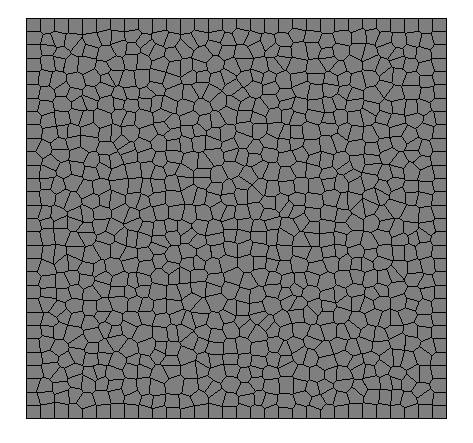
\includegraphics[width=1\textwidth]{figures/Amir_LEM_Domain_2D.png}
\subcaption{}
\label{fig:Amir_LEM_Domain_2D}
\end{subfigure}
\hfill
\begin{subfigure}[c]{0.48\textwidth}
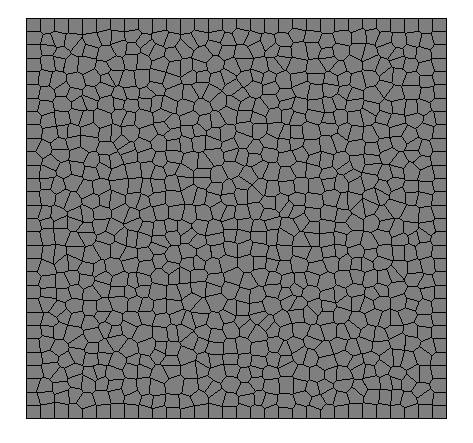
\includegraphics[width=1\textwidth]{figures/Amir_LEM_Domain_3D.png}
\subcaption{}
\label{fig:Amir_LEM_Domain_3D}
\end{subfigure}
\caption{The generated domain with $\alpha_{R} = 0.5$ (a) 2D discretization, and (b) 3D discretization}
\end{figure}

\subsubsection*{Mechanical lattice model}
\label{Section:MechanicalLattice}

The mechanical lattice model is based on the assumption of the Mode I and II linear elastic fracture mechanics. The simulation of the fracture in LEM is based on the removal of the bond elements between the neighboring Voronoi cells \cite{Rizvietal2019a}. The elements strength threshold is defined based on the critical strain energy or the fracture toughness for Mode I and II. In a different approach, the strength threshold is defined based on the Mohr-Coulombs tension cutoff model \cite{Bolanderetal1998}. The lattice elements are represented by a series of spring (1DOF),  Euler-Bernoulli beam (3DOF)(Figure \ref{fig:Amir_LEM_Beam}) or Timoshenko beam elements (4DOF). The regularization of the regular lattice model, such as a triangular or square discretization technique, is carried out and a relationship between the continuum and element properties is presented \cite{Ostojastarzewski2002, Karihalooetal2003}. This regularization assumes that the stored strain energy of a continuum, $U_{\mathbb{R}}$, is equal to the stored strain energies in each individual Voronoi cells, $U_{Cell}$. The strain energy stored in a unit cell depends on the total number of each cells bond elements ($N_b$), the elements response forces ($F_b$) and the response displacements ($u_b$). For a continuum, the stored energy depends on the continuum stresses ($\sigma_{\mathbb{R}}$) and continuum strains ($\varepsilon_{\mathbb{R}}$) throughout the continuum volume ($V_{\mathbb{R}}$).

\begin{figure}[!ht]
\centering
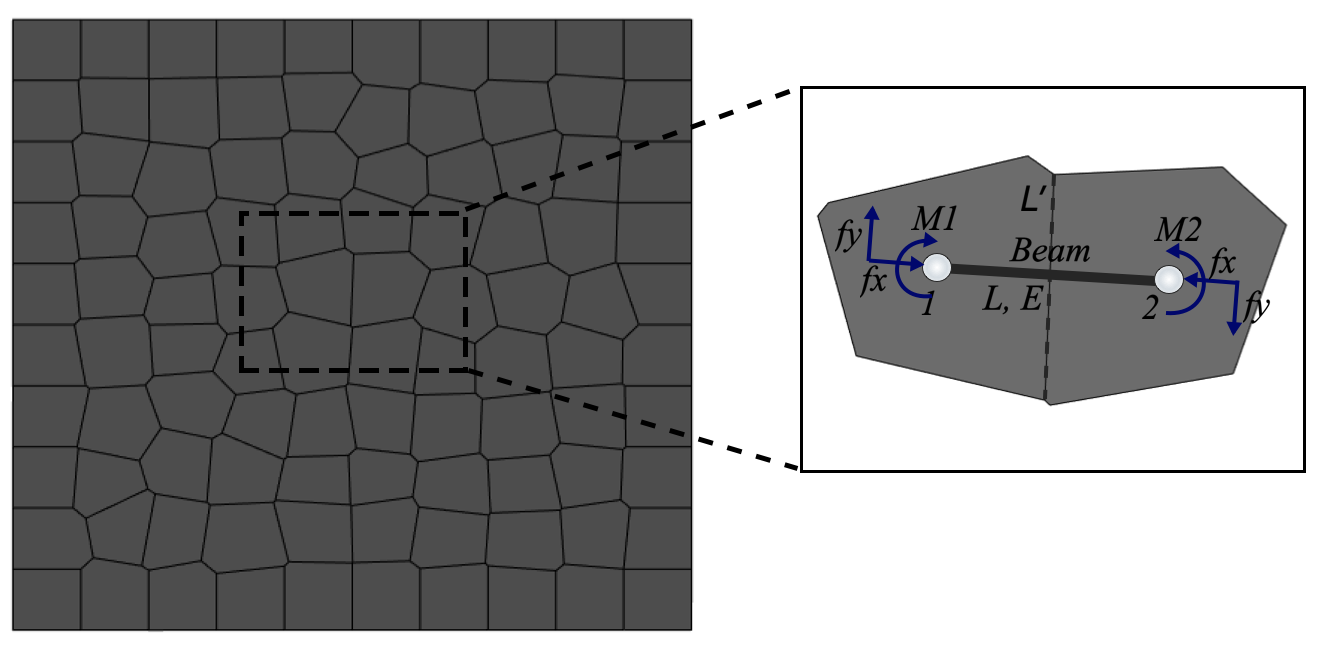
\includegraphics[width=0.75\textwidth]{figures/Amir_LEM_Beam.png}
\caption{The Euler-Bernoulli beam element representing the bond between two cells}
\label{fig:Amir_LEM_Beam}
\end{figure}

\begin{equation}
\label{eq:LEM_Mechanical_1}
 U_{Cell}=U_{\mathbb{R}}
\end{equation}

\begin{equation}
\label{eq:LEM_Mechanical_2}
 U_{Cell}=\frac{1}{2}\sum_{b=1}^{b=N_b}F_b.u_b
\end{equation}

\begin{equation}
\label{eq:LEM_Mechanical_3}
 U_{\mathbb{R}}=\frac{1}{2}\int_{V_{\mathbb{R}}}{\sigma_{\mathbb{R}}.\varepsilon_{\mathbb{R}}.dV}
\end{equation}

For a discretized 2D domain with the spring element, the length of the element ($L_b$), alignment orientation ($n_{i,j,k,m}$), first stiffness coefficient ($(R)^\prime$), continuum stiffness matrix $C_{\mathbb{R}}$, and strains of $\varepsilon_{i,j,k,m}$ are correlated as,

\begin{equation}
\label{eq:LEM_Mechanical_4}
U_{Cell}=\frac{1}{2}\sum_{b=1}^{b=N_b}L_b^2.((R)^\prime.n_i.n_j.n_k.n_m.\varepsilon_{ij}.\varepsilon_{km})_b
\end{equation}

\begin{equation}
\label{eq:LEM_Mechanical_5}
U_{\mathbb{R}}=\frac{1}{2}\varepsilon_{\mathbb{R}}.C_{\mathbb{R}}.\varepsilon_{\mathbb{R}}
\end{equation}

For a Euler-Bernoulli beam element in 2D, the curvature strain ($\kappa_{i,j}$), curvature stiffness ($D_{i,j}$), stiffens matrix ($C_{i,j,k,m}$) and second stiffness coefficient ($(R)^{\prime\prime}$) are related as,

\begin{equation}
\label{eq:LEM_Mechanical_6}
U_{\mathbb{R}}=\frac{V}{2}\varepsilon_{ij}C_{ijkm}\varepsilon_{km}+\frac{V}{2}\kappa_{i}D_{ij}\kappa_j
\end{equation}

\begin{equation}
\label{eq:LEM_Mechanical_7}
C_{ijkm}=\sum_{b=1}^{b=N_b} ({n_i.n_k \left( n_j.n_m.(R)^\prime)+n_j.n_m.(R)^{\prime\prime} \right)})_b
\end{equation}


After the regularization of the lattice model and with the minimization of the potential energy of the system, the load Vs. displacement relation in each time step is determined. For a single element, the stored total strain energy ($U_t^b$) is equal to the sum of axial ($U_a^b$), shear ($U_s^b$) and moment ($U_m^b$) strain energies. Eventually, the total strain energy depends on the axial force ($f_x$), shear force ($f_y$) and moment ($M_b$) along the element's length of $z=0:L_b$, the area of elements ($A_b$), element's shear modulus ($G_b$), element's Young's modulus ($E_b$), and moment of inertia ($I_b$). The bi-linear softening scheme is implemented to model the quasi-brittle material behavior existing in rock and concrete geomaterials \cite{Inceetal2003}. The measured $E_b$ values depends on the peak strain ($\varepsilon_p$), failure  strain ($\varepsilon_f$), current element strain ($\varepsilon_b$) and peak load ($f_p$) where the stiffness degradation starts.

\begin{equation}
\label{eq:LEM_Mechanical_8}
 U_t^b(z)=U_a^b(z)+U_s^b(z)+U_m^b(z)=\frac{1}{2}\int_{0}^{L_b}{\left(\frac{f_x{(z)}^2}{E_b A_b}+\frac{f_y{(z)}^2}{G_b A_b}+\frac{M_b{(z)}^2}{E_b I_b}\right).dz} 
\end{equation}

\begin{equation}
\label{eq:LEM_Mechanical_9}
E_b=\frac{f_p}{\varepsilon_f-\varepsilon_p}\left(\frac{\varepsilon_f}{\varepsilon_b}-1\right)
\end{equation}

\subsubsection*{Thermo-mechanical lattice model}
\label{Section:ThermalLattice}

The thermo-mechanical lattice model is based on the weak coupling scheme between the thermal and mechanical models, which decreases the computational costs. The thermal lattice model is based on the discrete thermal lattice model (TDEM) \cite{Zhangetal2011, Fengetal2008}, where the Hertzian contact model is implemented to account for the heat conductance ($h_b$) between the particles. The axial compression force increment ($f_x$) results in higher thermal conductance between the particles, which eventually leads to a higher effective thermal conductivity ($K_{eff}$). The regularization of the thermal lattice model is based on the relationship between the heat conductivity of elements and the continuum \cite{Rizvietal2018b}. The $h_b$ depends on the contact length ($L_b^\prime$) (or area in 3D domain), contact forces and assigned elements thermal conductivities ($k_{b}$).

\begin{equation}
\label{eq:LEM_Thermal_1}
h_b = k_{b} \left( (L_b^\prime)+ \left(\frac{3f_x L_b}{4E_b}\right)^\frac{1}{3} \right)
\end{equation}

In a steady state, the amount of the heat in- and outflow ($q_b$) from a Voronoi cell (Figure\ref{fig:Amir_LEM_Thermal}) is equal to zero,

\begin{figure}[!ht]
\centering
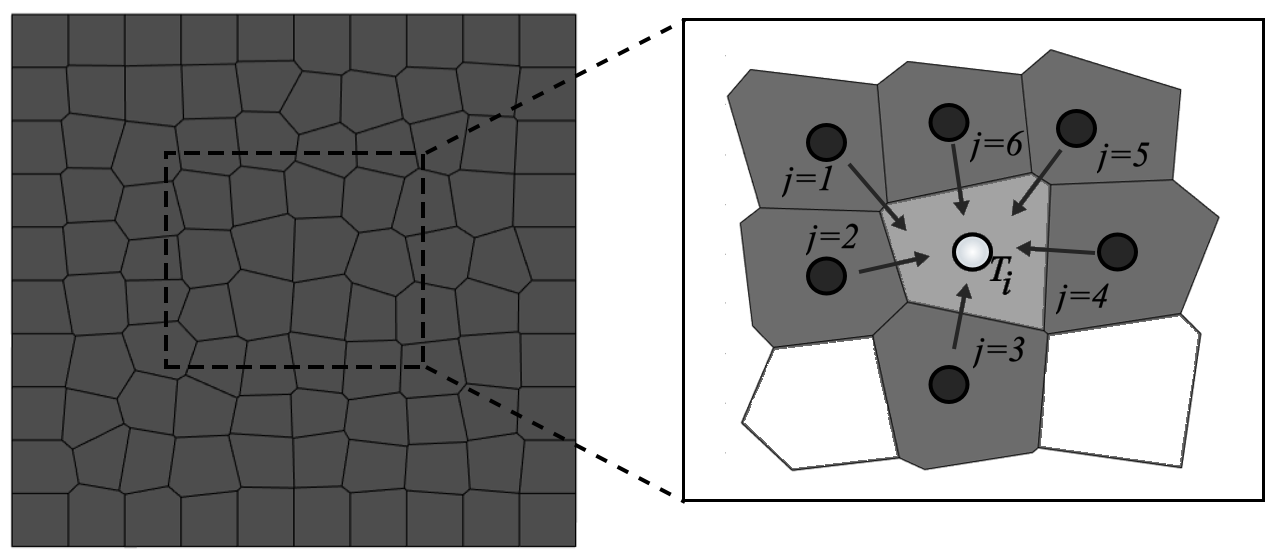
\includegraphics[width=0.75\textwidth]{figures/Amir_LEM_Thermal.png}
\caption{The heat flow into $i_{th}$ cell from surrounding boundaries}
\label{fig:Amir_LEM_Thermal}
\end{figure}


\begin{equation}
\label{eq:LEM_Thermal_2}
\rho_{i}c_{i}v_{i}\frac{dT_{i}}{dt}-\nabla .\left(k_i\nabla T_i\right)-\rho_i{\dot{q}}_i=0
\end{equation}

\begin{equation}
\label{eq:LEM_Thermal_3}
\nabla .\left(k\nabla T_i\right)=\sum_{b=1}^{b=N_b}{q_b}=\sum_{b=1}^{b=N_b}{h_b(T_i - T_j)_b=0}
\end{equation}

 
where, $\dot{q}$ is heat density (assumption: $\dot{q}=0$), $t$ is time, $\rho_{i}$ is density, $c_{i}$ is heat capacity and $v_{i}$ is the volume of each Voronoi cell ($i$). In a transient case,

\begin{equation}
\label{eq:LEM_Thermal_4}
\sum_{b=1}^{b=N_b}{q_b=}\rho_{i}c_{i}v_{i}\frac{dT_i}{dt}
\end{equation}

The effective thermal conductivity is calculated based on the average volume technique, where $q_{ave}$ is the average heat flow, $q_{Cell}^{b}$ is the heat flow through the assigned cells located in the boundary ($N_C$), $\dot{T}$ is the temperature gradient and  $\hat{x}_{cell}$ is the relative coordinates of each cell.

\begin{equation}
\label{eq:LEM_Thermal_5}
q_{ave}=\frac{\sum_{b=1}^{b=N_C}q_{Cell}^b.\hat{x}_{Cell}}{V}
\end{equation}

\begin{equation}
\label{eq:LEM_Thermal_6}
q_{ave}=K_{eff}.\dot{T}
\end{equation}

The thermal strain is calculated based on the linear expansion of the lattice elements and the given heat expansion coefficient. The implementation of the thermal expansion into the mechanical model results in a fully coupled thermo-mechanical model \cite{Sattarietal2019b}.

\subsubsection*{Hydro-mechanical lattice model} \label{Section:HMLattice}

The existing hydro-mechanical lattice models are based on the assumption of the dual lattice network, where the mechanical lattice elements transfer the mechanical loads between the two nodes and the conduct elements perpendicular to the alignment of the mechanical elements transfer the fluid or gas flow between the conduct nodes \cite{Grassl2009, Grassletal2013}. The implemented hydro-mechanical lattice model is based on the mass conservation ($m_f$) of the fluids in the continuum. The hydraulic aperture ($a_h$), fluid density ($\rho_f$),  fluid viscosity ($\nu_f$), flow length ($L_b^\prime$), hydraulic resistance ($R_h$), saturation degree ($Sr$) and bulk modulus ($K_f$) are the main parameters used to determine the hydraulic pressures ($P_f$) and transferred fluid masses ($\Delta m_f$) between the conduct nodes. 

\begin{equation}
\label{eq:LEM_Hydro_1}
m_f^{t+1}=m_f^t+\Delta m_f
\end{equation}

\begin{equation}
\label{eq:LEM_Hydro_2}
m_f^{t=0}={\rm Sr}^{t=0}V_{cav}\rho_f\left(1+\frac{P_f^{t=0}}{K_f}\right)
\end{equation}

\begin{equation}
\label{eq:LEM_Hydro_3}
\Delta m_{f,ij}=f\left(Sr\right).\frac{P_{f,j}-P_{f,i}-\rho_fg\left(Z_j-Z_i\right)}{R_h}.\Delta t
\end{equation}

where, $Z$ is the relative coordinate of the $i,j$ conduct nodes, $V_{cav}$ is the volume of the cavity, $g$ is the gravity and $f(Sr)$ is the saturation function which is equal to 0 and 1 in a dry and saturated conditions, respectively. According to the finite-discrete element method (FDEM) \cite{Lisjaketal2017}, the fluid mass is stored within defined physical and artificial cavities. Each conduct node represents an artificial cavity connected through conductive elements (Figure \ref{fig:Amir_LEM_Hydro}), where the hydraulic conductivity is governed based on the parallel plate cubic flow rule. 

\begin{figure}[!ht]
\centering
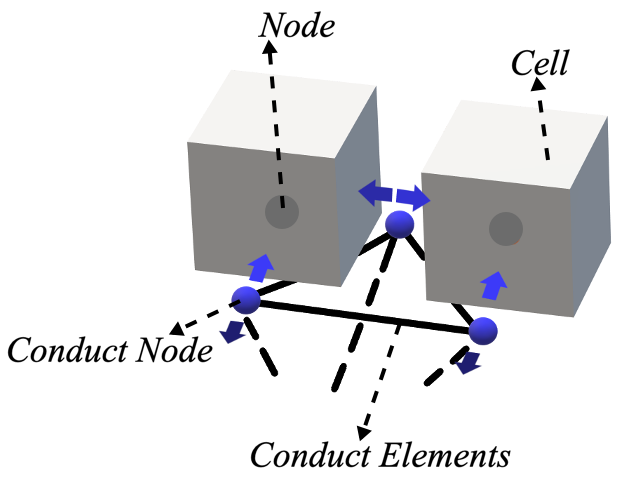
\includegraphics[width=0.75\textwidth]{figures/Amir_LEM_Hydro.png}
\caption{The schematic representation of the implemented hydro-mechanical model}
\label{fig:Amir_LEM_Hydro}
\end{figure}

\begin{equation}
\label{eq:LEM_Hydro_4}
R_h = \frac{12\nu_f}{a_h^3} L_b^\prime = 12 \nu_f \int_{z_i}^{z_j} \frac{1}{a_h (z^3)}dz= \frac{6 \nu_f (a_{h,j}+a_{h,i})}{(a_{h,i} a_{h,j})^2} L_b^\prime
\end{equation}


When an artificial cavity is saturated, the amount of excessive fluid mass flowing inside the cavity builds the pore pressure, which then is transmitted into the mechanical nodes. If the cavity is not saturated, then the pore pressure is assumed to be zero. 

\begin{equation}
\label{eq:LEM_Hydro_5}
P_f^t=P_f^{t-1}+K_f\frac{\Delta m_f}{\rho_fV_{cav}^t}\ \ \ \ \ \ \ \ \ \ \ if\ \ \ \ {\rm Sr}^t=1
\end{equation}


With the implementation of the pore pressures into the mechanical lattice nodes, the pore pressure diffusion and the change of the hydraulic conductivity with the crack opening and closure are measured. The flow simulation is implemented under both the pressure- and flowrate-controlled boundary conditions.


\subsubsection*{Shrinkage and swelling lattice model} 
\label{Section:ShrinkageLattice}

The simulation of the shrinkage and swelling using the lattice element method is based on the particle shrinkage model \cite{Simaetal2013}, which is mainly considered in the discrete models. In contrast to the DEM, the shrinkage in LEM is implemented into the lattice elements (Figure \ref{fig:Amir_LEM_Shrinkage}). To do so, the interface elements are generated to represent the bond between the particles (\cite{Sattarietal2019b}). The shrinkage and swelling coefficients ($\alpha_s$) are temperature dependent. According to the initial water content ($\omega^{t=0}$) and the change of the water content during the shrinkage and swelling process, the linear strain in the lattice elements is determined and implemented into the mechanical model. 

\begin{figure}[!ht]
\centering
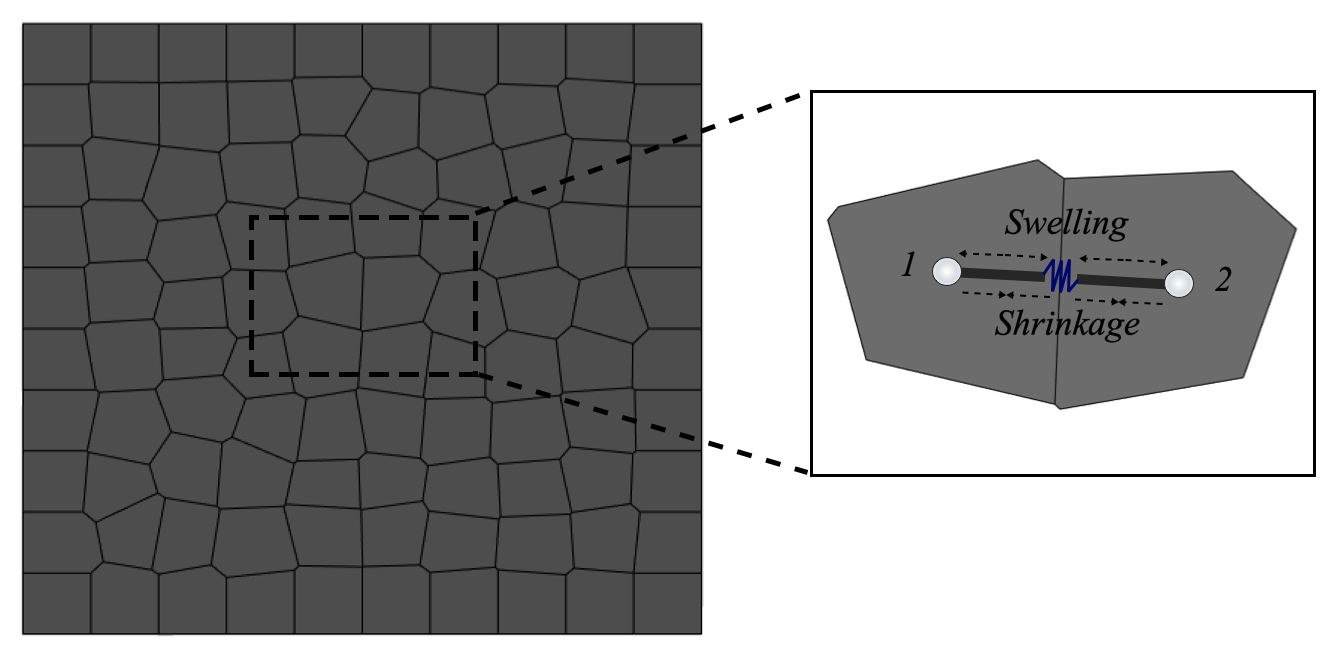
\includegraphics[width=0.75\textwidth]{figures/Amir_LEM_Shrinkage.png}
\caption{The implementation of the interface element to simulate the shrinkage and swelling processes}
\label{fig:Amir_LEM_Shrinkage}
\end{figure}

\begin{equation}
\label{eq:LEM_Shrinkage_1}
L_b^t=L_b^{t=0}e^{-\alpha_s.\frac{t}{t=\infty}}
\end{equation}

\begin{equation}
\label{eq:LEM_Shrinkage_2}
\alpha_s=-\frac{1}{3}\ln{(1-\frac{\omega^{t=0}-\omega^{t}}{1+e_0}}.G_s)
\end{equation}


The shrinkage and swelling coefficient are time, temperature and depth dependent. Therefore, graphs representing the evaporation rate as well as the soil water characteristic curves to assess the applied suction and the water content during the wetting and drying paths are required \cite{Voetal2017}. $\bar{\bar{\sigma}}$ and $\bar{\bar{\varepsilon}}$ are the stress and strain tensors, respectively. 

\begin{equation}
\label{eq:LEM_Shrinkage_3}
\bar{\bar{\sigma}}=C:\bar{\bar{\varepsilon}}-Sr.P_f\bar{\bar{\delta}}
\end{equation}

The elements shrinkage and expansion results in the axial compression and tensile stresses in the lattice elements, which when they exceed their predefined strength threshold are removed, is simulated as well as the micro fracking process under shrinkage and swelling conditions.
